%%%%%%%%%%%%%%%%%%%%%%%%%%%%%%%%%%%%%%%%%%%%%%%%%%%%%%%%%%%%%%%%%%%%%%%
%%%%%%%%%%%%%%%%%%%%%%%%%%%%%%%%%%%%%%%%%%%%%%%%%%%%%%%%%%%%%%%%%%%%%%% 
%%%%%%%%%%%       								 Preamble				         	                                                        %%%%%%%%%% 
%%%%%%%%%%%%%%%%%%%%%%%%%%%%%%%%%%%%%%%%%%%%%%%%%%%%%%%%%%%%%%%%%%%%%%% 
%%%%%%%%%%%%%%%%%%%%%%%%%%%%%%%%%%%%%%%%%%%%%%%%%%%%%%%%%%%%%%%%%%%%%%% 
\documentclass[10pt]{beamer}
\usepackage{setspace}
\usepackage{color}
\usepackage{amsmath,lmodern}
\usepackage{hyperref}
\usepackage{graphicx}
\usepackage{multirow}
\usepackage{tikz}
\usetikzlibrary{fit,shapes.misc}
\usepackage{pdflscape}
\usepackage{amsmath}
\usepackage{lscape}
\usepackage{multirow}
\usepackage{enumerate}
\usepackage{mathtools}
\usepackage{epstopdf}
\usepackage{pdfpages}
\usepackage{bm}
\usepackage{appendixnumberbeamer}
\usepackage{color,soul}
\usepackage{grffile}
\usepackage{float}
\usepackage{relsize}
\usepackage{tcolorbox}
\newcounter{nodemarkers}
\usepackage{tikz}
\newcommand{\toplinesmall}{%
  \tikz[remember picture,overlay] {%
    \draw[blue,thick] ([yshift=-1cm, xshift=.9cm]current page.north west)
             -- ([yshift=-1cm,xshift=3.6cm]current page.north west);}}
             
\newcommand{\toplinemedium}{%
  \tikz[remember picture,overlay] {%
    \draw[blue,thick] ([yshift=-1cm, xshift=.9cm]current page.north west)
             -- ([yshift=-1cm,xshift=6.2cm]current page.north west);}}
 
 \newcommand{\toplinelarge}{%
  \tikz[remember picture,overlay] {%
    \draw[blue,thick] ([yshift=-1cm, xshift=.9cm]current page.north west)
             -- ([yshift=-1cm,xshift=8.9cm]current page.north west);}}           
             
 \newcommand{\toplinexlarge}{%
  \tikz[remember picture,overlay] {%
    \draw[blue,thick] ([yshift=-1cm, xshift=.9cm]current page.north west)
             -- ([yshift=-1cm,xshift=12cm]current page.north west);}}                       
             
\setbeamertemplate{footline}
{
  \leavevmode%
  \hbox{%
  \begin{beamercolorbox}[wd=.333333\paperwidth,ht=2.25ex,dp=1ex,center]{author in head/foot}%
    \usebeamerfont{author in head/foot}{\textcolor{blue}{ECON712}}
  \end{beamercolorbox}%
  \begin{beamercolorbox}[wd=.333333\paperwidth,ht=2.25ex,dp=1ex,center]{title in head/foot}%
    \usebeamerfont{title in head/foot}{\textcolor{blue}{Winter 2026}}
  \end{beamercolorbox}%
  \begin{beamercolorbox}[wd=.333333\paperwidth,ht=2.25ex,dp=1ex,right]{date in head/foot}%
    \usebeamerfont{date in head/foot}{\textcolor{blue}{Lecture 6 \: \: \: \: \: \: \: }
    \insertframenumber{} / \inserttotalframenumber\hspace*{2ex}} 
  \end{beamercolorbox}}%
  \vskip0pt%
}
\newtheorem{proposition}[theorem]{Proposition}

\newcommand\marktopleft[1]{%
    \tikz[overlay,remember picture] 
        \node (marker-#1-a) at (-0.2,1.2ex) {};%
}
\newcommand\markbottomright[1]{%
    \tikz[overlay,remember picture] 
        \node (marker-#1-b) at (0.16,-1ex) {};%
    \tikz[overlay,remember picture,thick,inner sep=4pt]
        \node[draw,rectangle,rounded corners, blue, fit=(marker-#1-a.center) (marker-#1-b.center)] {};%
}

\setbeamertemplate{caption}{\raggedright\insertcaption\par}
\setbeamertemplate{itemize items}[ball]
\setbeamertemplate{itemize subitem}[triangle]
\setbeamertemplate{itemize subsubitem}[triangle]
\tcbset{colframe=white,colback=white,nobeforeafter}
\beamertemplatenavigationsymbolsempty
\addtobeamertemplate{frametitle}{\vspace*{0.19cm}}{\vspace*{0cm}}


%%%%%%%%%%%%%%%%%%%%%%%%%%%%%%%%%%%%%%%%%%%%%%%%%%%%%%%%%%%%%%%%%%%%%%%
%%%%%%%%%%%%%%%%%%%%%%%%%%%%%%%%%%%%%%%%%%%%%%%%%%%%%%%%%%%%%%%%%%%%%%% 
%%%%%%%%%  									    Define Title									                                       %%%%%%%%%
%%%%%%%%%%%%%%%%%%%%%%%%%%%%%%%%%%%%%%%%%%%%%%%%%%%%%%%%%%%%%%%%%%%%%%%
%%%%%%%%%%%%%%%%%%%%%%%%%%%%%%%%%%%%%%%%%%%%%%%%%%%%%%%%%%%%%%%%%%%%%%% 
\title{ECON 712: Applied Econometrics} 
\author{Lecture 6: Linear Regression using Vector Spaces, part II}
\date{}
\AtBeginSection[]
{
 \begin{frame}<beamer>
 \tableofcontents[currentsection]
 \end{frame}
}
%%%%%%%%%%%%%%%%%%%%%%%%%%%%%%%%%%%%%%%%%%%%%%%%%%%%%%%%%%%%%%%%%%%%%%%
%%%%%%%%%%%%%%%%%%%%%%%%%%%%%%%%%%%%%%%%%%%%%%%%%%%%%%%%%%%%%%%%%%%%%%% 
%%%%%%%% 						     				Document								                                                %%%%%%%%
%%%%%%%%%%%%%%%%%%%%%%%%%%%%%%%%%%%%%%%%%%%%%%%%%%%%%%%%%%%%%%%%%%%%%%%
%%%%%%%%%%%%%%%%%%%%%%%%%%%%%%%%%%%%%%%%%%%%%%%%%%%%%%%%%%%%%%%%%%%%%%% 
\begin{document}
\setbeamercovered{transparent}

\begin{frame}
\maketitle
\end{frame}

\begin{frame}
\frametitle{\: \: \: Vector Space Definitions} 
\toplinelarge
\begin{itemize}
\item We use set of vectors to formally define the following subspaces:
\begin{enumerate}
\vspace{0.11in}
\item $k$-dimensional subspace: 
\begin{eqnarray*}
\mathcal{S}(\bm{x_1},\bm{x_2},\cdots,\bm{x_k}) \equiv \left\{\bm{z}\in E^n \mathlarger{|} \bm{z}=\mathlarger{\sum}_{i=1}^{k}b_i \: \bm{x_i}, b_i \in  \mathbb{R} \right\}
\end{eqnarray*}
\vspace{0.11in}
\item $(n-k)$-dimensional orthogonal complement:  
\begin{eqnarray*}
\mathcal{S}^\perp(\bm{w})\equiv\left\{\bm{w} \in E^n \mathlarger{|} \bm{w}^T \: \bm{z}=0 \text{  for all} \bm{z}\in \mathcal{S}(\bm{x_1},\bm{x_2},\cdots,\bm{x_k})\right\}
\end{eqnarray*}
\end{enumerate}
\vspace{0.11in}
\item We will also make use of the following inequality, called Cauchy-Schwartz:
\begin{eqnarray*}
\langle \bm{x},\bm{y} \rangle \leq \|\bm{x}\|  \|\bm{y}\|
\end{eqnarray*}
\end{itemize}
\end{frame}

\begin{frame}
\frametitle{\: \: \: Linear Regression} 
\toplinelarge
\begin{itemize}
\item Linear Regression considers each linearly-independent $k$ column vector of size $n$ from $\bm{X}$ as the basis vector that spans the k-dimensional space
\begin{itemize}
\vspace{0.11in}
\item We also assume the following two conditions:
\begin{eqnarray*}
\begin{array}{lll}
\bm{X}^T \bm{\hat{u}}=\bm{0} &,   & \bm{y}=\bm{X} \bm{\hat{\beta}}+\bm{\hat{u}}
\end{array}
\end{eqnarray*}
\item This result in linear regression being defined as selecting $\bm{\hat{\beta}}$ that reaches the perpendicular dropped from $\bm{y}$ vector into the plane spanned by $\bm{X}$  
\end{itemize}
\end{itemize}
\end{frame}

\begin{frame}
\frametitle{\: \: \: Linear Regression} 
\toplinemedium
 \begin{figure}
\caption{Example with $n=3$, $k=2$}
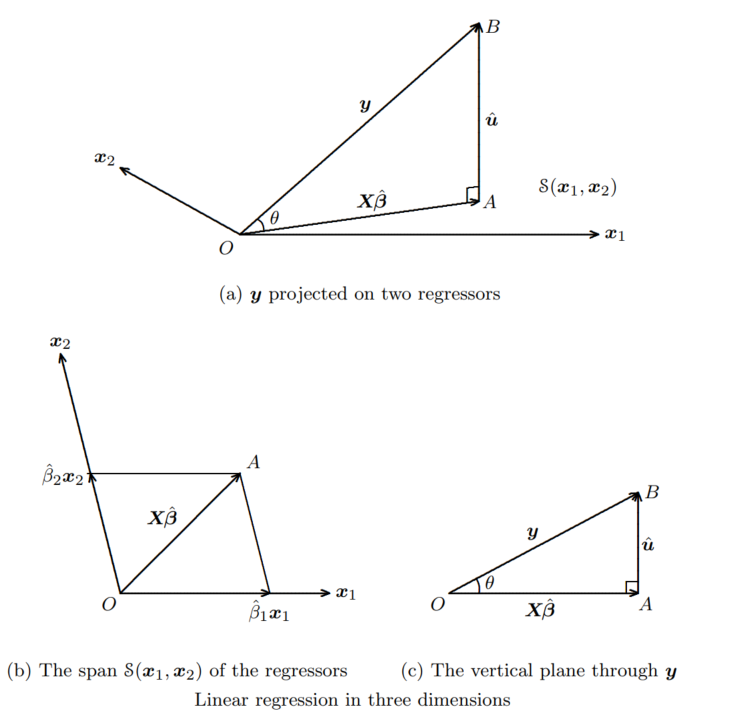
\includegraphics[scale=0.34]{linear_regression.png}
\end{figure}
\end{frame}

\begin{frame}
\frametitle{\: \: \: Linear Regression} 
\toplinemedium
\begin{itemize}
\item The concept of a dropping a perpendicular is formalized by an orthogonal projection:
\begin{eqnarray*}
\begin{array}{lll}
\bm{P_X}=\bm{X}(\bm{X}^T\bm{X})^{-1}\bm{X}^T &, & \bm{X}\bm{\hat{\beta}}=\bm{P_X \: y} 
\end{array}
\end{eqnarray*}
\begin{itemize}
\item An orthogonal projection is a matrix that projects any vector to a point in the subspace $\mathcal{S}(\bm{X})$ that it is closest to it
\vspace{0.11in}
\item $\mathcal{S}(\bm{X})$ is called the invariant subspace of $\bm{P_X}$ because the projection of any vector in $\mathcal{S}(\bm{X})$ using $\bm{P_X}$ leaves that vector unchanged
\end{itemize}
\vspace{0.11in}
\item We are also going to use a projection onto the orthogonal subspace of $\mathcal{S}(\bm{X})$, $\mathcal{S}^\perp$
\begin{eqnarray*}
\begin{array}{lll}
\bm{M_X}=\bm{I}-\bm{P_X} &, & \bm{\hat{u}}=\bm{M_X \: y}
\end{array}
\end{eqnarray*}
\end{itemize}
\end{frame}   

\begin{frame}
\frametitle{\: \: \: Linear Regression} 
\toplinemedium
\begin{itemize}
\item Important properties of the projection matrices:
\begin{enumerate}
\item Idempotent: 
\begin{eqnarray*}
\begin{array}{ll}
\bm{P_X} \: \bm{P_X}&=\bm{P_X} \\[2ex]
\bm{M_X} \: \bm{M_X}&=\bm{M_X}\\[2ex]
\end{array}
\end{eqnarray*}
\item Annihilation: $\bm{P_X} \: \bm{M_X}=\bm{M_X} \: \bm{P_X}=\bm{0}$ 
\end{enumerate}
\vspace{0.11in}
\item Also, by Pythagorean Theorem (Sum Squares):
\begin{eqnarray*}
\|\bm{y}\|^2=\|\bm{P_X \: y}\|^2+\|\bm{M_X \: y}\|^2
\end{eqnarray*}
\end{itemize}
\end{frame}

\begin{frame}
\frametitle{\: \: \: Linear Transformations} 
\toplinelarge
\begin{itemize}
\item Let $\bm{A}$ be a $kxk$ matrix with full rank, and define $\bm{Z}=\bm{X \: A}$ then :
\begin{eqnarray*}
\bm{A}\bm{\hat{\alpha}}=\bm{\hat{\beta}}
\end{eqnarray*}
where $\bm{X}\bm{\hat{\beta}}=\bm{P_X \: y}$, $\bm{Z}\bm{\hat{\alpha}}=\bm{P_Z \: y}$
\vspace{0.11in}
\item There are two cases (can be combined as in the Celsius/Fahrenheit example in ETM):
\begin{enumerate}
\vspace{0.11in}
\item When the regressors are multiplied by a constant (e.g. change of units from cm to meters)
\vspace{0.11in}
\item When a constant is added/subtracted from regressors
\end{enumerate} 
\end{itemize}
\end{frame}

\begin{frame}
\frametitle{\: \: \: Linear Transformations} 
\toplinelarge
\begin{itemize}
\item Subtracting a constant $\bm{\iota}c$ from regressors when the constant term is included
\end{itemize}
\begin{figure}
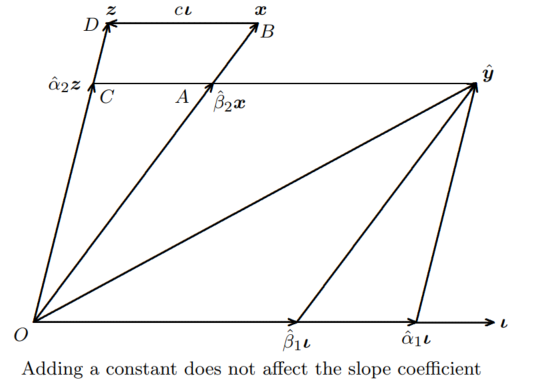
\includegraphics[scale=0.54]{constant.png}
\end{figure}
\end{frame}

\begin{frame}
\frametitle{\: \: \: Linear Transformations} 
\toplinelarge
\begin{itemize}
\item Subtracting a constant $\bm{\iota}\bar{x}$ from regressors when the constant term is included
\end{itemize}
\begin{figure}
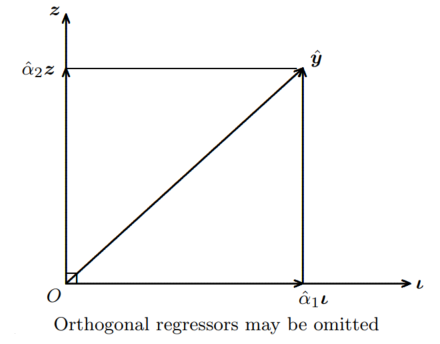
\includegraphics[scale=0.55]{average.png}
\end{figure}
\end{frame}

\end{document}